% Options for packages loaded elsewhere
\PassOptionsToPackage{unicode}{hyperref}
\PassOptionsToPackage{hyphens}{url}
\PassOptionsToPackage{dvipsnames,svgnames,x11names}{xcolor}
%
\documentclass[
]{article}
\title{Syntax 2021/2022}
\author{Teodor Petrič}
\date{2021-10-11}

\usepackage{amsmath,amssymb}
\usepackage{lmodern}
\usepackage{iftex}
\ifPDFTeX
  \usepackage[T1]{fontenc}
  \usepackage[utf8]{inputenc}
  \usepackage{textcomp} % provide euro and other symbols
\else % if luatex or xetex
  \usepackage{unicode-math}
  \defaultfontfeatures{Scale=MatchLowercase}
  \defaultfontfeatures[\rmfamily]{Ligatures=TeX,Scale=1}
\fi
% Use upquote if available, for straight quotes in verbatim environments
\IfFileExists{upquote.sty}{\usepackage{upquote}}{}
\IfFileExists{microtype.sty}{% use microtype if available
  \usepackage[]{microtype}
  \UseMicrotypeSet[protrusion]{basicmath} % disable protrusion for tt fonts
}{}
\makeatletter
\@ifundefined{KOMAClassName}{% if non-KOMA class
  \IfFileExists{parskip.sty}{%
    \usepackage{parskip}
  }{% else
    \setlength{\parindent}{0pt}
    \setlength{\parskip}{6pt plus 2pt minus 1pt}}
}{% if KOMA class
  \KOMAoptions{parskip=half}}
\makeatother
\usepackage{xcolor}
\IfFileExists{xurl.sty}{\usepackage{xurl}}{} % add URL line breaks if available
\IfFileExists{bookmark.sty}{\usepackage{bookmark}}{\usepackage{hyperref}}
\hypersetup{
  pdftitle={Syntax 2021/2022},
  pdfauthor={Teodor Petrič},
  colorlinks=true,
  linkcolor={Maroon},
  filecolor={Maroon},
  citecolor={Blue},
  urlcolor={Blue},
  pdfcreator={LaTeX via pandoc}}
\urlstyle{same} % disable monospaced font for URLs
\usepackage[margin=1in]{geometry}
\usepackage{longtable,booktabs,array}
\usepackage{calc} % for calculating minipage widths
% Correct order of tables after \paragraph or \subparagraph
\usepackage{etoolbox}
\makeatletter
\patchcmd\longtable{\par}{\if@noskipsec\mbox{}\fi\par}{}{}
\makeatother
% Allow footnotes in longtable head/foot
\IfFileExists{footnotehyper.sty}{\usepackage{footnotehyper}}{\usepackage{footnote}}
\makesavenoteenv{longtable}
\usepackage{graphicx}
\makeatletter
\def\maxwidth{\ifdim\Gin@nat@width>\linewidth\linewidth\else\Gin@nat@width\fi}
\def\maxheight{\ifdim\Gin@nat@height>\textheight\textheight\else\Gin@nat@height\fi}
\makeatother
% Scale images if necessary, so that they will not overflow the page
% margins by default, and it is still possible to overwrite the defaults
% using explicit options in \includegraphics[width, height, ...]{}
\setkeys{Gin}{width=\maxwidth,height=\maxheight,keepaspectratio}
% Set default figure placement to htbp
\makeatletter
\def\fps@figure{htbp}
\makeatother
\setlength{\emergencystretch}{3em} % prevent overfull lines
\providecommand{\tightlist}{%
  \setlength{\itemsep}{0pt}\setlength{\parskip}{0pt}}
\setcounter{secnumdepth}{5}
\usepackage{booktabs}
\usepackage{amsthm}
\makeatletter
\def\thm@space@setup{%
  \thm@preskip=8pt plus 2pt minus 4pt
  \thm@postskip=\thm@preskip
}
\makeatother
\ifLuaTeX
  \usepackage{selnolig}  % disable illegal ligatures
\fi
\usepackage[]{natbib}
\bibliographystyle{plainnat}

\begin{document}
\maketitle

{
\hypersetup{linkcolor=}
\setcounter{tocdepth}{2}
\tableofcontents
}
\hypertarget{einfuxfchrung}{%
\section{Einführung}\label{einfuxfchrung}}

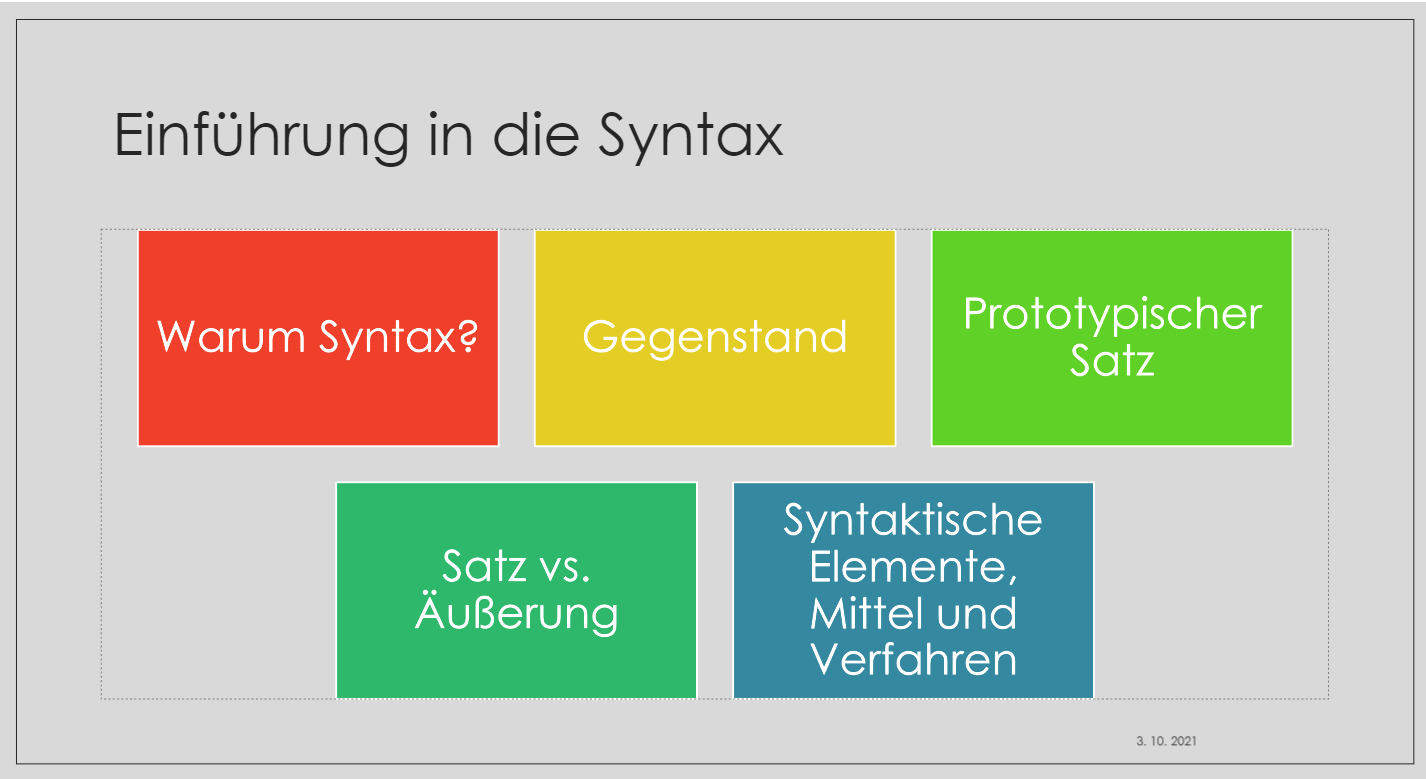
\includegraphics[width=1\linewidth]{pictures/Syntax_intro_01}

In diesem Einführungskurs machen wir Sie mit grundlegenden Methoden zur
Erfassung von linguistischen, insbesondere aber syntaktischen Merkmalen
in deutschen und slowenischen Texten bekannt.

Unseren Kurs beginnen wir mit Frage, wozu wir überhaupt über Sprache
reden und \emph{zu welchem Zweck über Syntax?}

Da sich mehrere Wissenschaften mit Sprache auseinandersetzen, ist es
sinnvoll, Syntax von anderen wissenschaftlichen Disziplinen abzugrenzen,
um den \emph{Gegenstand der Syntax} (als Bestandteil der Systemlinguistik)
besser erkennen zu können.

In jeder wissenschaftlichen Disziplin werden grundlegende Einheiten
definiert. In der Syntax ist der \emph{Satz} die maßgebliche Basiseinheit.
Wie jede linguistische Einheit, kann man Sätze verschiedentlich
definieren. Im Rahmen der Einführungsstunde wird ein \emph{prototypischer
Satz} definiert. Von der syntaktischen Einheit \emph{Satz} ist die
kommunikative Einheit \emph{Äußerung} zu unterscheiden.

Andere Themen im Verlauf der Einführung in die deutsche Syntax sind
\emph{syntaktische Elemente, syntaktische Mittel und Verfahren zur Ermittlung
syntaktischer Einheiten} wie etwa der Satztypen, Satzglieder und
Attribute.\footnote{Dieses Buch wurde mit \texttt{Bookdown} \citep{xie2015} verfasst.}

Hinweise\footnote{Clipart von \url{https://www.clipartmax.com/}}:

Das ist eine Definition (rmdnote).

Das ist ein Tip oder eine Info (rmdtip).

Das ist ein Arbeitsvorschlag (rmdrobot).

Das ist der RStudio Logotyp (rmdrstudio).

Das ist eine Warnung (rmdwarning).

Das ist eine Fehlermeldung (rmderror).

\hypertarget{gegenstand-und-sinn-der-syntax}{%
\section{Gegenstand und Sinn der Syntax}\label{gegenstand-und-sinn-der-syntax}}

Im Alltag, sei es privat oder im Beruf, verständigen wir uns vorrangig mit Hilfe von mündlich oder schriftlich geführten Texten. Will man den Aufbau eines Textes besser kennen lernen, ist es sinnvoll, ihn nach nachvollziehbaren Prinzipien und Methoden in kleinere Einheiten zu zerlegen. In der Sprachwissenschaft hat sich eine längere Liste von Einheiten in Texten etabliert, die man verschiedenen Bereichen zuordnen kann. Hier sollen vor allem diejenigen Bereiche erwähnt werden, die gemeinsam die Grammatik einer Sprache umreißen.

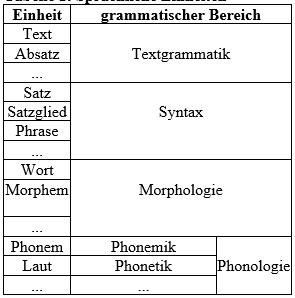
\includegraphics[width=1\linewidth]{pictures/grammatische_bereiche}

Der \emph{Text} ist die umfangreichste und hierarchisch höchste kommunikative Einheit, die aus inhaltlich zusammenhängenden \emph{Äußerungen} besteht und eine nachvollziehbare und sortenspezifische Struktur aufweist (Engel 1988: 33).

\hypertarget{uxe4uuxdferung}{%
\subsection{Äußerung}\label{uxe4uuxdferung}}

\emph{Sprachliche Äußerung}:
sinnvolle Lautfolge zwischen zwei Pausen
Inhalt Absicht

Äußerung
Satzförmig \textless--\textgreater{} nicht-satzförmig

\texttt{Äußerungen} lassen sich als Laut- oder Schriftzeichenketten definieren, die von einem Sprecher zwischen zwei Pausen produziert werden und aus einem oder mehreren Sätzen bestehen können (Bußmann 21990: 52). Im Gegensatz zu Sätzen sind sie \emph{kommunikative} Einheiten und gehören somit auf die Ebene der \emph{Performanz} oder Parole. \texttt{Sätze} sind hingegen Einheiten des Sprachsystems und gehören somit auf die Ebene der \emph{Kompetenz} oder Langue.

\emph{Äußerungen} können die Form (d.h. die Struktur, den Aufbau) von Sätzen (z.B. Hauptsätzen) oder satzförmigen Konstruktionen (z.B. Nebensätzen, Infinitivgruppen) haben, oder auch nicht-satzförmig (z.B. als Nominalphrase) auftreten (vgl. Engel 1988: 33).

\hypertarget{prototypischer-satz}{%
\subsection{Prototypischer Satz}\label{prototypischer-satz}}

\emph{Prototypischer Satz}
- Finites Verb
- Eignen sich dazu, Sprechhandlungen eindeutig auszudrücken
- Enthält kein unterordnendes Element (z.B. keinen Subjunktor)

Die \emph{Syntax} gilt traditionell als Lehre vom Satzbau. Sie ist ein Teilbereich der Grammatik natürlicher Sprachen und bildet ein System von Regeln, die beschreiben, wie aus einem Inventar von Grundelementen (d.h. Morphemen, Wörtern, Satzgliedern) durch spezifische syntaktische Mittel (d.h. morphologische Markierung, Intonation, Reihenfolge) alle wohlgeformten Sätze einer Sprache abgeleitet werden können (nach Bußmann 21990: 766).

\hypertarget{syntaktische-grundbeziehungen}{%
\subsection{Syntaktische Grundbeziehungen}\label{syntaktische-grundbeziehungen}}

In den folgenden Abschnitten sollen die folgenden syntaktischen Grundbeziehungen beschrieben werden:

\begin{enumerate}
\def\labelenumi{\arabic{enumi}.}
\tightlist
\item
  die zwei Seiten eines sprachlichen Zeichens - Inhalt vs.~Ausdruck
\item
  paradigmatische vs.~syntagmatische Beziehungen zwischen sprachlichen Zeichen
\item
  Konstituenzbeziehungen zwischen sprachlichen Zeichen
\item
  Dependenzbeziehungen zwischen sprachlichen Zeichen
\end{enumerate}

Jedes sprachliche Zeichen hat hat zwei Seiten:
• die \emph{Inhalts- oder Bedeutungsseite}
• die \emph{Ausdrucks- oder Formseite}.

Nur die \emph{Ausdrucksseite} ist direkt zugänglich, während die Inhaltsseite erschlossen werden muß. Die Form einer Münze z.B. können wir mit unseren Sinnen wahrnehmen, welche Bedeutung sie jedoch für uns hat, müssen wir erst mit Hilfe unseres gespeicherten Wissens u.a. erschließen.

In flektierenden bzw. fusionierenden Sprachen (z.B. Deutsch, Slowenisch) wird ein und derselbe Inhalt häufig durch verschiedene Formen ausgedrückt (vgl. derselbe Sachverhalt in Aktiv vs.~Passiv, verschiedene Suffixe für Personenbezeichnungen, verschiedene Suffixe für Plural usw.). Umgekehrt gilt, daß ein Ausdruck oft polyfunktional bzw. polysem ist, d.h. daß er je nach sprachlicher oder außersprachlicher Umgebung mehrere Bedeutungen auszudrücken vermag (vgl. die verschiedenen Funktionen der Suffixe -en oder -er, der Partikeln ja, doch, eben, denn, der Tempora Präsens oder Perfekt usw.). Eine eineindeutige Entsprechung (1:1 Entsprechung) zwischen Inhalt und Ausdruck besteht somit nicht. Agglutinierende Sprachen (z.B. Türkisch) nähern sich diesem ``Ideal'' (als eines ``Ideale'' gilt 1:1 Entsprechung zwischen Inhalt und Form deshalb, weil das Gedächtnis weniger belastet ist als bei 1:n Entsprechungen).

Mehr über die Beziehung zwischen Inhalt und Ausdruck ist aus den Folien über die Kodierverfahren zu ersehen.

Die \emph{syntaktische Form von Sätzen} verändert sich nach Eisenberg (1989: 45-47) auf verschiedene Weise:
• durch \emph{Variierung der Reihenfolge} von Satzelementen (Haben zwei Sätze dieselben Elemente und treten diese Satzelemente in verschiedener Reihenfolge auf, dann haben die beiden Sätze eine verschiedene Form, und zwar ohne Rücksicht auf Bedeutungsunterschiede oder Bedeutungsgleichheit der beiden Sätze);
• durch \emph{Intonation} (d.h. die Kombination aus Tonhöhe, Tondauer und Tonstärke) in der gesprochenen Sprache bzw. durch Interpunktion (d.h. Komma, Punkt, Doppelpunkt, usw.) in der geschriebenen Sprache (Die Intonation ist zweifellos ein Formmittel, denn man hört, auf welchem Satzelement der Hauptakzent liegt, oder ob die Tonhöhe am Satzende steigt);
• durch \emph{morphologische Veränderung} von Einheiten im Satz (Verändert man die im Satz vorkommenden Elemente durch Präfixe, Suffixe, Infixe, Umlaut oder Ablaut, verändert man auch die syntaktische Form eines Satzes).

``Dadurch daß eine linguistische Einheit in einem bestimmten Kontext vorkommen kann, können zweierlei Relationen entstehen. Sie steht in paradigmatischer Relation zu all jenen Einheiten, die gleichfalls in demselben Kontext vorkommen können (gleichgültig, ob sie mit der ersten Einheit kontrastieren oder in freier Variation sind) und in syntagmatischer Relation zu jenen anderen Einheiten derselben Stufe, mit denen zusammen sie vorkommt und die ihren Kontext bilden.'' (Lyons 71989: 75) \emph{Paradigmatische und syntagmatische Beziehungen} sind nicht nur auf syntaktischer Ebene, sondern auf allen Ebenen linguistischer Beschreibung bedeutend, also etwa auch auf phonologischer, morphologischer und semantischer Ebene (Lyons 71989: 76). Die Elemente, die ein Paradigma bilden, sind somit füreinander austauschbar und können nicht gleichzeitig stehen. Die Elemente, die ein Syntagma bilden, sind nicht füreinander austauschbar und kommen in demselben Kontext vor. Elemente in syntagmatischer Beziehungen bilden eine Struktur. Die Zahl der möglichen Strukturen ist theoretisch gesehen unendlich. Ein Paradigma oder System ist hingegen eine endliche Menge von Wahlmöglichkeiten, die dem Sprecher in einem bestimmten Kontext zur Verfügung stehen. Syntagmatische und paradigmatische Beziehungen werden zur Veranschaulichung oft in einem zweidimensionalen Koordinatensystem abgebildet. Auf der horizontalen Achse werden die syntagmatischen Beziehungen und auf der vertikalen Achse die paradigmatischen Beziehungen abgebildet. Die horizontale Achse wird auch als Strukturachse und die vertikale Achse auch als Systemachse oder Wahlachse bezeichnet (z.B. eine Satzstruktur mit Pronominalparadigma zur Veranschaulichung einzeichnen).

Speziell in der Syntax bestehen \emph{syntagmatische} Beziehungen zwischen Konstituenten (d.h. Einheiten eines Satzes). Für das Deutsche setzt Eisenberg (1989: 52) \emph{vier Typen} solcher Beziehungen an, und zwar \emph{Rektion}, \emph{Identität}, \emph{Kongruenz} und \emph{Positionsbezug}.

\begin{enumerate}
\def\labelenumi{\arabic{enumi}.}
\tightlist
\item
  \emph{Rektion}
\end{enumerate}

Der Begriff Rektion (lat. regere „regieren``; engl. government; slow. vezavnost) wird in Abhängigkeit von der jeweiligen Grammatiktheorie verschieden verwendet. Das regierende Element wird als Regens, das von ihm abhängige Element dagegen als Rektum oder Dependens bezeichnet. In der traditionellen Grammatik sprach man von Rektion, wenn der Kasus eines Objektes vom Verb abhängig war.

\begin{enumerate}
\def\labelenumi{(\arabic{enumi})}
\tightlist
\item
  Verb: essen : Kinder essen gern {[} akk Pfannkuchen{]}.
\item
  Präposition: zu : Morgen muß ich zu{[}m Zahnarzt dat{]}.
\item
  Nomen: Anweisung : die Anweisung {[} gen meines Chefs{]}
\end{enumerate}

Konstituenten, die durch Rektionsbeziehung miteinander verbunden sind, bilden zusammen eine höhere Konstituente. Beispiel: Ein Substantiv (Paradigmenkategorie SUBSTANTIV) kann ein Genitivattribut binden, regiert als den Genitiv und legt damit die Form des Attributes fest (das Haus meines Vaters).

In Konkurrenz zur Rektion steht der von Tesnière geprägte Valenzbegriff (engl. valency; slow. vezljivost). \emph{Valenz} ist ein der aus der Chemie entlehnter Begriff (vgl. die Fähigkeit von Atomkernen eine bestimmte Anzahl von Elektronen zu binden mit der Fähigkeit von bestimmten Lexemen eine bestimmte Anzahl von anderen Lexemen oder Wortgruppen zu binden).

Nach Helbig \& Buscha ist Valenz eine semantisch begründete Fähigkeit von lexikalischen Elementen (insbesondere Verben, Nomina, Adjektiven), Leerstellen im Satz zu eröffnen, die von Aktanten (d.h. Ergänzungen) besetzt werden können oder müssen. Nach Eisenberg ist Valenz eine besondere Form von Rektion.

\begin{enumerate}
\def\labelenumi{\arabic{enumi}.}
\setcounter{enumi}{1}
\tightlist
\item
  \emph{Identität}
\end{enumerate}

``Eine Konstituente f1 steht in der Identitätsbeziehung zu einer Konstituente f2, wenn es bestimmte grammatische Kategorien gibt, denen beide Konstituenten zugeordnet sind.'' (Eisenberg 21989: 54) Als Beispiel: koordinierte Nominalphrasen, enge Apposition: der Bürger Danton.

\begin{enumerate}
\def\labelenumi{\arabic{enumi}.}
\setcounter{enumi}{2}
\tightlist
\item
  \emph{Kongruenz}
\end{enumerate}

Unter Kongruenz versteht man im allgemeinen die formale Übereinstimmung einer Wortform mit einer anderen oder mit anderen Wortformen.

Kongruenzerscheinungen sind in den Sprachen der Welt verschieden geregelt. Übereinzelsprachlich häufig ist die Kongruenz zwischen dem Prädikat und dem Subjekt des Satzes, während andere Kongruenzerscheinungen (wie beispielsweise die Kongruenz zwischen Subjekt und adjektivischer Prädikatsergänzung) sprachspezifischer zu sein scheinen.

\begin{enumerate}
\def\labelenumi{(\arabic{enumi})}
\setcounter{enumi}{3}
\tightlist
\item
  {[}Der Elefant 3.P.Sg.{]} {[}trink-t 3.P.Sg.{]} Wasser. (Person und Numerus kongruieren)
\item
  {[}Slon 3.P.Sg. {]} {[}pi-je 3.P.Sg. {]} vodo. (Kongruenz hinsichtlich Person und Numerus)
\end{enumerate}

Im Deutschen gibt es zwar eine Kongruenz zwischen dem finiten Verb und dem Subjekt des Satzes, aber keine zwischen Subjekt und adjektivischer Prädikatsergänzung wie im Slowenischen (oder Italienischen).

\begin{enumerate}
\def\labelenumi{(\arabic{enumi})}
\setcounter{enumi}{5}
\tightlist
\item
  Der Verkäufer ist noch jung. vs.~Die Verkäuferin ist noch jung.
\item
  Prodajalec je še mlad. vs.~Prodajalka je še mlad-a.
\end{enumerate}

Selbst die Kongruenz zwischen Subjekt und finitem Verb ist verschieden ausgebildet, je nachdem in welcher Form das Subjekt des Satzes auftritt. Erscheint es im Deutschen als Nomen, kongruiert es mit dem finiten Verb eigentlich nur hinsichtlich Numerus, denn der Wert für die Personkategorie kann nicht variieren (es handelt sich immer um die dritte Person, d.h. die besprochene Person oder Sache); erscheint es im Deutschen dagegen als Pronomen, kann es mit dem finiten Verb auch hinsichtlich Person kongruieren, denn man kann statt der dritten Person auch die erste oder zweite einsetzen.

\begin{enumerate}
\def\labelenumi{(\arabic{enumi})}
\setcounter{enumi}{7}
\tightlist
\item
  Der Mechaniker repariert gerade meinen Wagen.
\item
  Er repariert gerade meinen Wagen. (3. Person Singular)
\item
  Der Mechaniker sagt: ``Ich repariere gerade ihren Wagen.'' (1. Person Singular)
\item
  Ich fragte den Mechaniker: ``Wann reparieren Sie meinen Wagen.'' (3. Person Plural)
\item
  Meine Freundin fragte mich: ``Reparierst du meinen Wagen oder soll ich lieber einen Fachmann damit beauftragen?'' (2. Person Singular)
\end{enumerate}

Da das Slowenische wie beispielsweise Italienisch eine sogenannte Pro-Drop-Sprache ist, sind Pronomen in der Funktion eines Subjekts nur dann obligatorisch, wenn man Sie aufgrund des Kontextes hervorheben möchte. Ansonsten werden thematische Subjektpronomen in der slowenischen Standardsprache nicht realisiert. In der Syntaxtheorie wird das nicht realisierte thematische Subjektpronomen als pro (kleingeschrieben !) notiert.

\begin{enumerate}
\def\labelenumi{(\arabic{enumi})}
\setcounter{enumi}{12}
\tightlist
\item
  {[}Subj Mehanik{]} popravlja pravkar moj avto.
\item
  Pravkar popravlja {[}Subj pro{]} moj avto. (3. Person Singular)
\item
  Mehanik reče: ``Pravkar popravljam {[}Subj pro{]} Vaš avto.'' (1. Person Singular)
\item
  Vprašam mehanika: ``Kdaj boste {[}Subj pro{]} popravili moj avto?'' (2. Person Plural)
\item
  Moja prijateljica me vpraša: ``Ali boš TI popravil moj avto ali naj raje pokličem strokovnjaka?'' (das Subjektpronomen wird realisiert und durch Kontrastbetonung hervorgehoben)
\end{enumerate}

Im Slowenischen kann das Subjekt zusätzlich mit dem infiniten Verb hinsichtlich der Genuskategorie kongruieren.

\begin{enumerate}
\def\labelenumi{(\arabic{enumi})}
\setcounter{enumi}{17}
\tightlist
\item
  Prodajalec je odprl trgovino.
\item
  Prodajalka je odprla trgovino.
\end{enumerate}

Wie oben gezeigt wurde, ist dies auch bei adjektivischen Prädikatsergänzungen der Fall. Im Gegenwartsdeutschen ist diese Kongruenzerscheinung nicht bekannt.

Traditionell wird noch ein weiterer Fall von formaler Übereinstimmung als Kongruenz behandelt, nämlich die formale Übereinstimmung zwischen dem Nomen und seinen vorangestellten Begleitern, den Adjektiven und Artikelwörtern. In der Grammatik von Eisenberg (21989) finden wir dazu eine andere Ansicht.

\begin{enumerate}
\def\labelenumi{\arabic{enumi}.}
\setcounter{enumi}{3}
\tightlist
\item
  \emph{Positionsbezug}
\end{enumerate}

``Eine Konstituente f1 ist positionsbezogen auf eine Konstituente f2, wenn die Position von f2 relativ zu f1 festliegt.'' (Eisenberg 21989: 56) Als Beispiele können uns die Konstruktionen Präposition + N; Subjunktor + V-Letzt-Stellung dienen.

In Abhängigkeit vom Sprachtyp werden Wortverbindungen nach vorgegebenen Stellungsregeln behandelt. In den sogenannten SVO-Sprachen, zu denen man das Englische, Französische und Slowenische aufgrund der charakteristischen Abfolge Subjekt vor Verb und Verb vor Objekt zählen könnte, gibt es eine Präferenz, einen regierten Ausdruck rechts vom Regens anzuordnen: z.B. das Akkusativobjekt rechts vom regierenden Verb oder die Nominalphrase rechts von der regierenden Präposition. Im Französischen ist die Rechts-Präferenz noch stärker ausgeprägt, denn Adjektive in einer Nominalphrase erscheinen rechts vom regierenden Nomen. In einer älteren Entwicklungsstufe der slawischen Sprachen soll dies ebenfalls der Fall gewesen sein (z.B. wie in oče naš).

\begin{enumerate}
\def\labelenumi{(\arabic{enumi})}
\setcounter{enumi}{19}
\tightlist
\item
  The shop assistant has opened {[} Obj the shop{]}.
\item
  Prodajalec je odprl {[} akkobj trgovino{]}.
\end{enumerate}

In Sprachen mit dominanter SOV-Anordnung (mit der Abfolge Subjekt vor Objekt und Verb-Letzt-Stellung), zu denen man das Gegenwartsdeutsche zählen könnte, ist eine umgekehrte Präferenz zu erwarten, nämlich daß der regierende Ausdruck links vom Regens angeordnet wird: z.B. das Akkusativobjekt links vom regierenden Verb oder die Nominalphrase links von der regierenden Präposition oder attributive Adjektive links vom regierenden Nomen. Tatsächlich stehen Akkusativobjekte (und andere Objekte), wenn Sie als Nominalphrasen ausgedrückt werden, vor dem regierenden Verb in Infinitiv- oder Partizipialform und attributive Adjektive erscheinen vor dem regierenden Nomen.

\begin{enumerate}
\def\labelenumi{(\arabic{enumi})}
\setcounter{enumi}{21}
\tightlist
\item
  Der Verkäufer hat soeben {[} akkobj das Geschäft{]} geöffnet.
\item
  {[}Der adj blonde N Verkäufer{]} hat soeben das Geschäft geöffnet.
\end{enumerate}

Was die Struktur der deutschen Präpositionalphrasen anbelangt, scheint die oben angestrebte Generalisierung nicht standzuhalten, denn es gibt im Deutschen viele Phrasen, in denen die Nominalphrase der regierenden Präposition folgt. Andererseits ist zu beobachten, daß es im Gegenwartsdeutschen in Einklang mit der Generalisierung auch Postpositionen gibt, d.h. Fügewörter, die der regierten Nominalphrase folgen und ihr nicht voranstehen.

\begin{enumerate}
\def\labelenumi{(\arabic{enumi})}
\setcounter{enumi}{23}
\tightlist
\item
  nach meiner Meinung vs.~meiner Meinung nach
\item
  entlang des Flusses vs.~den Fluss entlang
\end{enumerate}

Postpositionen sind in Sprachen mit dominanter SVO-Stellung selten oder überhaupt nicht vorhanden. An der Tatsache, dass im Deutschen sowohl Präpositionen als auch Postpositionen vorkommen, obwohl letztere präferent zu erwarten gewesen wären, zeigt sich andererseits, dass eine Sprache häufig einen Mischtyp verschiedener Kodierungsstrategien darstellt.

\begin{enumerate}
\def\labelenumi{\arabic{enumi}.}
\setcounter{enumi}{2}
\tightlist
\item
  \emph{KONSTITUENZ}
\end{enumerate}

Sprachliche Ausdrücke treten notgedrungenerweise linear in einem Satz auf, d.h. zeitlich oder räumlich nacheinander. Die Linearität der menschlichen Rede ist jedoch nicht das einzige Prinzip und bei weitem nicht das wichtigste. Dies zeigt sich an einfachen Sätzen wie Unsere Studenten haben die Pflichtlektüre nicht gelesen daran, daß für jeden kompetenten Sprecher der deutschen Sprache engere Beziehungen zwischen bestimmten Satzelementen offensichtlich sind: (a) zwischen unsere und Studenten, (b) zwischen haben und gelesen, (c) zwischen die und Pflichtlektüre und (d) zwischen Studenten und haben. Diese engeren Beziehungen zwischen den angeführten Satzelementen zeigen sich auch auf grammatischer Ebene: (a) beide Wörter stehen im Nominativ Plural, (b) die beiden Verbformen bilden zusammen eine Tempusform, die Perfekt genannt wird und sowohl Gegenwarts- als auch Vergangenheitsbezug hat, (c) beide Wörter stehen im Akkusativ Singular und sind feminine Formen, (d) die beiden Wörter kongruieren miteinander, d.h. hier sie stimmen in ihrer morphologischen Form bezüglich Person und Numerus überein (3. Person Plural). Die enge Beziehung der beiden Wörter in (b) zeigt, daß sprachliche Ausdrücke in engeren Beziehungen zueinander stehen können, selbst wenn sie weit auseinander stehen. Das oben angeführte Satzbeispiel offenbart, daß man neben der Linearität der menschlichen Rede mit weiteren grundlegenden Prinzipien zu rechnen hat, nämlich mit der Konstituenz und der Dependenz von Sätzen und ihren Teilen.

Konstituenz ist eine grundlegende syntaktische Beziehung bei der Beschreibung der hierarchischen Struktur von Sätzen oder deren Teilen. Zwischen zwei linear auftretenden sprachlichen Ausdrücken A und B besteht eine Konstituenzbeziehung, wenn beide von einem weiteren Element C dominiert werden. Dominanz zwischen zwei Elementen A und C liegt genau dann vor, wenn die Konstituente A eine Konstituente oder eine Teilkonstituente von C ist. Das Element C besteht somit aus den Bestandteilen A und B.

C

A B

In dem oben angeführten Satzbeispiel besteht die Nominalphrase Unsere Studenten (C) aus den Bestandteilen unsere (A) und Studenten (B) oder die Nominalphrase die Pflichtlektüre (C) aus den Konstituenten die (A) und Pflichtlektüre (B). Eine der beiden dominierten Konstituenten (A oder B) vererbt seine Eigenschaften (teilweise) an die dominierende Kategorie C.

Konstituenz ist einerseits vergleichbar mit einer Relation in der Semantik (Bedeutungslehre), nämlich der Beziehung zwischen einem Oberbegriff und den entsprechenden Unterbegriffen (d.h. zwischen einem Hyperonym und seinen Hyponymen): z.B. das Hyperonym Tier und seine Hyponyme Hund, Katze, Kuh, Pferd, Löwe, Zebra, Goldfisch usw. Die ``Vererbung'' der Eigenschaften an das Hyperonym richtet sich andererseits nach Gemeinsamkeiten zwischen den Hyponymen, wohingegen sich die Vererbung der Eigenschaften bei der syntaktischen Dominanzbeziehung nach den Eigenschaften des Kopfes der Phrase richtet (Kopfprinzip) und nicht nach den gemeinsamen Eigenschaften der Elemente der Phrase.

An dieser Stelle soll auch die Bedeutung der oben verwendeten Begriffe Kategorie und Phrase erläutert werden. Eine Phrase ist eine Verbindung von Satzelementen (z.B. Wörtern), die gemeinsam an eine andere Stelle im Satz verschoben werden können. Wenn beispielsweise von einer Nominalphrase die Rede ist, dann ist eine Wortverbindung aus der lexikalischen Kategorie Nomen und seinen (fakultativen) Begleitern (z.B. Adjektiven) gemeint, in der das Nomen den Kopf der Phrase darstellt, was daran ersichtlich ist, daß die gesamte Phrase die Eigenschaften der lexikalischen Kategorie Nomen übernimmt (``erbt''). Die Bestandteile der Nominalphrase unsere Studenten im oben verwendeten Satz können aufgrund ihrer Zusammengehörigkeit gemeinsam an eine andere Stelle im Satz verschoben werden (z.B. Die Pflichtlektüre haben unsere Studenten nicht gelesen), während einzelne Teile der Nominalphrase diese Fähigkeit gewöhnlich nicht haben (z.B. *Die Pflichtlektüre haben Studenten nicht unsere gelesen).

Wenn in diesem Zusammenhang von Kategorie die Rede ist, sind grammatische Kategorien gemeint. Laut Bußmann (1990: 291-292) sind grammatische Kategorien Abstraktionsklassen linguistischer Einheiten, d.h. im Rahmen des Strukturalismus ``Klassen von sprachlichen Ausdrücken, die bezüglich eines bestimmten Kontextes unter Wahrung der Grammatikalität füreinander ersetzbar sind'', im Rahmen der generativen Transformationsgrammatik ``Klassen von Ausdrücken, die bestimmte Strukturstellen im Satz ausfüllen können''. Traditionell versteht man darunter morphologische Kategorien (z.B. Person, Numerus, Genus) und syntaktische Kategorien (z.B. die Wortarten Nomen, Verb, Adjektiv usw., die phrasalen Kategorien Nominalphrase, Verbalphrase, Adjektivalphrase usw.). Die Wortarten (z.B. Nomen, Adjektiv, Adverb, Verb) werden übrigens auch als lexikalische Kategorien bezeichnet im Gegensatz zu den Wortverbindungen, die dann als phrasale Kategorien eingeordnet werden (z.B. Nominalphrase, Adjektivalphrase, Verbalphrase, Adverbialphrase). Von den lexikalischen und phrasalen Kategorien sind die syntaktischen Funktionen (z.B. Subjekt, Akkusativobjekt, Adverbialbestimmung) zu unterscheiden, d.h. grammatische Relationen, die außerhalb der Konstituente in Bezug auf andere Teile des Satzes (etwa des Verbs) bestimmt werden. Ein und dieselbe lexikalische oder phrasale Kategorie kann in Sätzen verschiedene syntaktische Funktionen haben. Im oben verwendeten Satz Unsere Studenten haben die Pflichtlektüre nicht gelesen hat die Nominalphrase Unsere Studenten die Funktion eines Subjekts (die man mit Wer oder was? erfragen kann), im Satz Dort sehe ich unsere Studenten hat dieselbe Nominalphrase die Funktion eines Akkusativobjekts (das man mit Wen oder was? erfragen kann). Da syntaktische Funktionen wie beispielsweise Subjekt, Objekt oder Adverbialbestimmung Relationscharakter haben, lassen sich nicht isoliert vom Kontext aufzählen wie beispielsweise die Wortklassen Nomen, Adjektiv oder Verb. Ein Adjektiv kann im Satz verschiedene Funktionen ausüben: es kann als Begleiter eines Nomens (das ist die sogenannte Attributfunktion) oder als Ergänzung zum Verb (das ist die sogenannte Prädikativfunktion, in Valenzmodellen auch Adjektivalergänzung genannt) auftreten.

\begin{enumerate}
\def\labelenumi{\arabic{enumi}.}
\setcounter{enumi}{3}
\tightlist
\item
  \emph{DEPENDENZ}
\end{enumerate}

Als Grundbeziehung zwischen (linear auftretenden) sprachlichen Elementen gilt auch das Prinzip der Dependenz, d.h. der Abhängigkeit eines Elementes von einem anderen. Sprachliche Elemente stehen somit wie andere Erscheinungen in unserer Welt in Hierarchiebeziehungen zueinander. Das abhängige Element wird Dependens genannt, das nicht-abhängige dagegen Regens (vgl. syntagmatische Beziehung Rektion). Die Dependenz ist eine syntaktische Grundbeziehung, bei der ein Element (das Dependens) nicht ohne ein anderes (das Regens) auskommen kann: z.B. in der Phrase ziemlich wichtige Persönlichkeiten kann die Partikel ziemlich nicht ohne das Adjektiv wichtig auftreten, da die Phrase *ziemlich Persönlichkeiten keine wohlgeformte Phrase der deutschen Sprache wäre (also ungrammatisch). Das Dependenzprinzip steht in den sogenannten Valenzgrammatiken bzw. Valenzmodellen im Mittelpunkt. Die Satzstruktur wird hierarchisch gegliedert, mit dem Verb (Verbalkomplex, Prädikat) an der Spitze. Derartige Valenzmodelle werden übrigens als Valenzverbgrammatiken bezeichnet. Über das Dependenzprinzip soll später noch im Vergleich mit der Konstituentengrammatik und im Rahmen des Valenzmodells gesprochen werden.

\hypertarget{identifikationsverfahren}{%
\subsection{Identifikationsverfahren}\label{identifikationsverfahren}}

\emph{Identifikationsverfahren}
1. Verschiebeprobe
2. Austauschprobe, Ersatzprobe (Fragetest)
3. Eliminierungsprobe
4. Hinzufuegungsprobe
(5. Koordinationsprobe, Häufungsprobe, Akzentuierungsprobe mit Satz- oder Kontrastakzent)

\begin{enumerate}
\def\labelenumi{\arabic{enumi}.}
\tightlist
\item
  Die \emph{Verschiebeprobe} wird auch Umstellprobe oder Permutationsprobe genannt. Dieses Verfahren dient dazu, Konstituenten eines Satzes zu ermitteln. Konstituenten des Satzes kann man in vielen Fällen mit der Kategorie Satzglied gleichsetzen. Ein Ausdruck, der aus einem oder mehreren Wörtern besteht, wird als Konstituente eines Satzes bezeichnet, wenn er sich im Satz frei verschieben läßt.
\end{enumerate}

(1a) Der Professor hält einen Vortrag über Textlinguistik.
(1b) Einen Vortrag über Textlinguistik hält der Professor.

Die unterstrichene Phrase in (1a) läßt sich frei im Satz verschieben, z.B. an den Anfang des Satzes. Der Satz ist trotz der Verschiebung der unterstrichen Phrase grammatisch richtig (2b). Daraus können wir folgern, daß die unterstrichene Phrase eine Konstituente des Satzes ist.

Nun folgt ein Beispiel, in dem die unterstrichene sprachliche Einheit keine Satzkonstituente ist.

(2a) Der Professor hält einen Vortrag über Textlinguistik.
(2b) *Einen hält der Professor Vortrag über Textlinguistik.

Das unterstrichene sprachliche Element in (2a) läßt sich nicht frei im Satz verschieben. Stellt man es z.B. an den Anfang des Satzes, erhält man einen ungrammatischen Satz (2b). Daraus folgern wir, daß das unterstrichene sprachliche Element keine Konstituente des Satzes ist. Es kann höchstens Teil einer Konstituente des Satzes sein.

2a. Die \emph{Kommutationsprobe} ist eine Substitutions- oder \emph{Ersetzungsprobe}. Dieses Verfahren dient dazu, Konstituenten mit gleicher Funktion im Satz festzustellen. Lassen sich zwei oder mehrere Ausdrücke füreinander austauschen, dann haben sie die gleiche Funktion im Satz.

\begin{enumerate}
\def\labelenumi{(\arabic{enumi})}
\setcounter{enumi}{2}
\tightlist
\item
  Der Professor hält einen Vortrag über Textlinguistik.
  der Mann
  der Dozent
  die Frau
  Der da vorne
  die Studentin
  er
  sie
  \ldots{}
  Die untereinander stehenden Ausdrücke haben im Satz die gleiche Funktion. Man sagt, sie kommutieren miteinander. Miteinander kommutierende Ausdrücke bilden ein Paradigma (auch als System bezeichnet).
\end{enumerate}

2b. Die \emph{Anaphorisierungsprobe} ist eine Substitutions- oder \emph{Ersetzungsprobe}. Dieses Verfahren dient dazu, die Satzgliedklasse festzustellen, der eine Satzkonstituente angehört. Anaphern sind Ausdrücke, die auf einen Ausdruck im Vortext hinweisen. Das Pronomen er in (4) bezieht sich auf der Professor im davorstehenden Satz.

\begin{enumerate}
\def\labelenumi{(\arabic{enumi})}
\setcounter{enumi}{3}
\tightlist
\item
  Der Professor hält einen Vortrag über Textlinguistik. Er hat auch mehrere Bücher zu diesem Themenbereich veröffentlicht.
\end{enumerate}

Der Ausdruck Professor kommutiert außerdem mit einer speziellen Anapher, und zwar mit dem Pronomen er. Dies bedeutet, daß man das Wort Professor in ein und demselben Satz durch das Pronomen er ersetzen kann (5). Das ist deshalb möglich, weil sie im Satz dieselbe Satzgliedfunktion haben.

\begin{enumerate}
\def\labelenumi{(\arabic{enumi})}
\setcounter{enumi}{4}
\tightlist
\item
  Der Professor hält einen Vortrag über Textlinguistik.
  Er
\end{enumerate}

Für jede Satzgliedklasse (Ergänzungsklasse) kann man im Prinzip eine spezielle Anapher finden. Auf diese Weise ist eine Satzgliedklassifizierung möglich. Die Anaphorisierungsprobe wirkt so wie die Kommutationsprobe entlang der paradigmatischen Achse (y-Achse).

2c. Die \emph{Fragewortprobe} ist ebenfalls eine Ersetzungsprobe. Sie dient wie die Anaphorisierungsprobe der Ermittlung der Satzgliedklasse. Eine Konstituente des Satzes wird in einer durch ein entsprechendes Fragewort ersetzt, d.h. man versucht die betreffende Konstituente zu erfragen.

(6a) Der Professor hält einen Vortrag über Textlinguistik.
(6b) Wer hält einen Vortrag über Textlinguistik?
(6c) Der Professor hält einen Vortrag worüber?
(6d) Worüber hält der Professor einen Vortrag?

Die Fragewortprobe ist allerdings etwas schwieriger zu handhaben, weil sie gleichzeitig die Umstellung (Verschiebung) von Satzgliedern notwendig macht. Die Fragewortprobe besteht genau genommen aus zwei Tests: (a) der Verschiebeprobe (siehe 6d) und (b) dem Einsetzen eines entsprechenden Fragewortes. (a) ist ein syntagmatischer Test, (b) hingegen ein paradigmatischer.

\begin{enumerate}
\def\labelenumi{\arabic{enumi}.}
\setcounter{enumi}{2}
\tightlist
\item
  Die Eliminierungsprobe (auch \emph{Weglaßprobe} oder \emph{Tilgungsprobe} genannt) dient zur Ermittlung von obligatorischen und fakultativ auftretenden Konstituenten des Satzes. In der Valenzgrammatik wird betont, daß die Unterscheidung zwischen Ergänzungen und Angaben mit ihr nicht möglich ist.
\end{enumerate}

(6a) Der Professor hält einen Vortrag über Textlinguistik.
(6b) *Der Professor hält über Textlinguistik.
(7a) Der Professor spricht mit seinen Studenten über Textlinguistik.
(7b) Der Professor spricht mit seinen Studenten.
(7c) Der Professor spricht über Textlinguistik.
(7d) Der Professor spricht.

In (6b) sehen wir, daß das Verb halten obligatorisch eine Akkusativergänzung verlangt (einen Vortrag), während das bedeutungsähnliche Verb sprechen fakultative Ergänzungen aufweist (7). Läßt man obligatorische (d.h. syntaktisch notwendige) Ergänzungen weg, erhält man einen ungrammatischen Satz. Ist eine Ergänzung lediglich fakultativ (d.h. syntaktisch nicht notwendig), bleibt der Satz grammatisch richtig.

Manchmal wird die sogenannte \emph{Reduktionsprobe} von der Tilgungsprobe unterschieden. Während bei der Tilgungsprobe eine beliebige Konstituente weggelassen wird, insofern der Satz dadurch nicht ungrammatisch wird, können bei der Reduktionsprobe auch syntaktisch notwendige Konstituenten weggelassen werden. Während das weggelassene Element nach der Tilgungsprobe nicht mehr zu rekonstruieren ist, kann das weggelassene Element nach der Reduktionsprobe noch rekonstruiert werden, d.h. daß der Hörer in der Lage ist, die ausgelassene Konstituente zu ergänzen (vgl. Wöllstein-Leisten\&Heilmann\&Stepner\&Vikner 1997: 16).

\begin{enumerate}
\def\labelenumi{(\arabic{enumi})}
\tightlist
\item
  {[}Das Wasser{]} kocht. / {[}Es{]} kocht.  * \_\_ kocht.
\item
  Hühner essen {[}Eier{]}, Menschen essen {[}Eier{]}.  Hühner essen \_\_, Menschen essen Eier.
\end{enumerate}

Ergibt sich wie in (2) eine elliptische Konstruktion, so wurde nur eine Konstituente getilgt.

\begin{enumerate}
\def\labelenumi{\arabic{enumi}.}
\setcounter{enumi}{3}
\tightlist
\item
  \emph{Hinzufügungsprobe}
\end{enumerate}

Das Gegenteil der Tilgungsprobe.

\begin{enumerate}
\def\labelenumi{\arabic{enumi}.}
\setcounter{enumi}{4}
\tightlist
\item
  \emph{Koordinationsprobe}
\end{enumerate}

Wenn sich zwei oder mehrere Elemente eines Satzes durch eine koordinierende Konjunktion (wie und oder oder) verbinden lassen, bilden sie eine Konstituente.
(1) {[}{[}Die Studenten{]} und {[}Professoren{]}{]} machen eine gemeinsame Exkursion.
(2) {[}Der eine freut sich{]} und {[}der andere ärgert sich{]}.
(3) eine {[}reizvolle{]} und {[}intelligente{]} Frau

Andere Tests:
Häufung, Akzentuierungsprobe (Satzakzent, Kontrastakzent)

\emph{Häufung}

Bestimmte Ausdrücke (etwa Partikeln) können gehäuft werden, d.h. sie können gleichzeitig im Satz auftreten, ohne daß sie durch eine koordinierende Konjunktion (z.B. und) miteinander verbunden werden könnten, ohne daß sie frei im Satz verschiebbar wären (wie etwa Konstituenten im Satz) oder gemeinsam im Satz verschiebbar wären (wie etwa Bestandteile von Konstituenten).

\begin{enumerate}
\def\labelenumi{(\arabic{enumi})}
\tightlist
\item
  Der Junge hat ja eben keinen Hunger.
\item
  *Der Junge hat ja und eben keinen Hunger.
\item
  *Ja hat der Junge eben keinen Hunger.
\item
  *Eben hat der Junge ja keinen Hunger.
\item
  *Ja eben hat der Junge keinen Hunger.
\end{enumerate}

\emph{Akzentuierung}

Durch entsprechende Akzentuierung und Herstellung eines entsprechenden Kontextes zeigt sich erst, ob eine bestimmte Satzform in einer Sprache möglich ist.

Nachdem vier grundlegende Verfahren zur Identifizierung von Satzkonstituenten und ihrer Rolle im Satz vorgeführt wurden, soll in den nächsten Absätzen einige der möglichen \emph{Schwierigkeiten} gezeigt werden, die \emph{bei der Verwendung dieser Verfahren} auftreten können. Die Verschiebeprobe liefert beispielsweise nicht in allen Fällen eindeutige Ergebnisse, d.h. man kann mit ihr nicht immer eindeutig nachweisen, daß ein sprachliches Element keine Konstituente des Satzes ist. In (3) ist dieses Problem veranschaulicht.

(3a) Der Professor hält einen Vortrag über Textlinguistik.
(3b) Über Textlinguistik hält der Professor einen Vortrag.

Die unterstrichene Präpositionalphrase in (3a) läßt sich frei im Satz verschieben, z.B. an den Anfang des Satzes. Ist diese Phrase dann etwa auch eine Konstituente des Satzes? Die Verschiebeprobe legt dies nahe. Dagegen spricht allerdings das Dependenzprinzip (ein semantisch begründetes Prinzip), denn man kann zeigen, daß die Präpositionalphrase über Textlinguistik vom Nomen Vortrag regiert (verlangt) wird und nicht vom Verb halten. Das Nomen Vortrag fordert folgende Ergänzungen: eine Person, die vorträgt, und einen Gegenstand, der von der Person vorgetragen wird. Die handelnde Person wird als Satzsubjekt am Satzanfang genannt und braucht daher nicht als Genitivattribut in der Nominalphrase wiederholt zu werden, der Gegenstand des Vortrags in der Präpositionalphrase. Das Verb halten fordert ebenfalls eine handelnde Person (als Subjekt im Satz) und einen Gegenstand, fordert allerdings im Gegensatz zum Nomen Vortrag, daß der Gegenstand als Nomen im Akkusativkasus realisiert wird:

\begin{verbatim}
vgl. halten <(Person: nom), (Gegenstand: akk)> 
vs. Vortrag <(Person: gen), (Gegenstand: prp)>. 
\end{verbatim}

Die Präpositionalphrase über Textlinguistik kann demnach nicht der geforderte Gegenstand sein, sondern nur die Nominalphrase einen Vortrag, die im Akkusativ steht. Umgekehrt könnten wir die Präpositionalphrase über Textlinguistik in (3) auch durch die Nominalphrase die Textlinguistik ersetzen, weil ein ungrammatischer Satz entstehen würde. Die Kommutationsprobe (d.h. der Austausch der Präpositionalphrase durch eine Nominalphrase) zeigt somit, zwischen welchen Teilen des Satzes engere Abhängigkeitsbeziehungen bestehen. Das Abhängigkeitsprinzip legt demnach über die Valenzbeziehungen zwischen den Satzelementen nahe, daß die Präpositionalphrase über Textlinguistik keine unmittelbare Konstituente des Satzes, sondern lediglich eine unmittelbare Konstituente der Nominalphrase mit dem Nomen Vortrag ist. Einen Teil einer Satzkonstituente (oder eines Satzgliedes) nennt man auch ein Attribut. Die Eliminierungsprobe unterstützt in diesem Fall das Ergebnis, das die Kommutationsprobe erbracht hat, denn sie zeigt, daß die ausgelassene Nominalphrase ein obligatorischer Bestandteil des Satzes ist, während dies für die Präpositionalphrase nicht zutrifft: Läßt man nämlich einen Vortrag in (3) aus, dann erhalten wir einen ungrammatischen Satz (3c).

(3a) Der Professor hält einen Vortrag über Textlinguistik.
(3c) *Über Textlinguistik hält der Professor.

Die Nominalphrase einen Vortrag (samt Präpositionalattribut über Textlinguistik) ist somit eine obligatorische Ergänzung des Verbs. Daß die Ergänzung einen Vortrag obligatorisch im Satz mit dem Verb halten vorkommen muß, zeigt die Eliminierungsprobe.

Die semantischen und syntaktischen Verhältnisse in (3) liegen allerdings noch komplizierter, denn bei genauerer Überlegung sieht man, daß das Nomen Vortrag und das Verb halten zusammen das Prädikat des Satzes bilden, d.h. semantisch eine Einheit bilden. Beide Varianten haben die Grundbedeutung: ``etwas vor einem Auditorium sprachlich vermitteln''. Das kann man nachweisen, indem man beide Ausdrücke durch einen Ausdruck ersetzt, und zwar Vortrag halten durch vortragen. Wenn Vortrag und halten nun gemeinsam das Prädikat bilden, könnte man die Präpositionalphrase über Textlinguistik dennoch für eine unmittelbare Konstituente des Satzes halten. Dann wäre auch verständlich, warum sich die Präpositionalphrase frei im Satz verschieben läßt.

Versucht man nun das einfache Verb vortragen in (3) statt des komplexen Ausdrucks einen Vortrag halten einzusetzen, stößt man jedoch auf Schwierigkeiten. Die beiden Varianten haben zwar dieselbe Grundbedeutung (4), das einfache Verb ist jedoch nicht in (3) einsetzbar.

(3a) Der Professor hält einen Vortrag über Textlinguistik.
(3d) *Der Professor trägt über Textlinguistik vor.
(3e) Der Professor trägt einen Text vor.

Das einfache Verb ist nicht in (3) einsetzbar, weil es eine andere syntaktische Valenz hat. Es fordert nämlich (wie das Verb halten) keine Präpositionalphrase als Objekt (3d), sondern eine Nominalphrase mit einem Nomen im Akkusativ Text (3e). Die Äußerung (3a) zeigt im Vergleich mit (3e) auch einen kleinen, aber wichtigen semantischen Unterschied, der parallel zum syntaktischen verläuft: Verwendet man das komplexe Prädikat einen Vortrag halten, dann nennt man in der Präpositionalphrase den Bereich, über den gesprochen wird. Verwendet man hingegen das einfache Verb vortragen, dann nennt man im Akkusativkasus den Gegenstand und nicht den Bereich. Der Gegenstand in (3e) ist ein Text, d.h. eine inhaltlich zusammenhängende Folge von Äußerungen. Dieser Text kann schriftlich fixiert sein und damit auch in konkreter Form auf Papier vorliegen. Der Bereich ist ein abstrakterer Gegenstand als der Text. Er ließe sich allenfalls mit einer Skizze konkretisieren.

Der Vergleich von (3a) mit (3f) ergibt noch einen weiteren syntaktischen und gleichzeitig semantischen Unterschied.

(3a) Der Professor hält einen Vortrag über Textlinguistik.
(3f) Der Professor trägt einen Text über Textlinguistik vor.

Das einfache Verb vortragen hat zwar dieselbe Grundbedeutung wie einen Vortrag halten (siehe oben), aber das komplexe Prädikat einen Vortrag halten enthält noch ein weiteres semantisches Merkmal, nämlich das Merkmal Gegenstand. Dieses Merkmal wird durch das Nomen Vortrag realisiert. Der Vortrag läßt sich ja genau genommen paraphrasieren als ``Text, der vorgetragen wird''. Dies bedeutet, daß der Begriff ein Text in das Wort Vortrag hineinverlegt (inkorporiert) worden ist. Demnach ist es richtiger, das komplexe Prädikat einen Vortrag halten mit dem komplexen Prädikat einen Text vortragen zu paraphrasieren (3g):

(3a) Der Professor hält einen Vortrag über Textlinguistik.
(3g) Der Professor trägt einen Text über Textlinguistik vor.

Die Äußerung (3a) mit dem Nominalisierungsverbgefüge einen Vortrag halten entpuppt sich damit als verkürzender Ausdruck für das morphologisch komplexe (und außerdem auch trennbare) Verb vortragen und dessen Akkusativobjekt einen Text. Will der Sprecher lediglich den Bereich nennen, über den die Rede ist, verwendet er das Nominalisierungsverbgefüge. Wenn er aber den konkreten Text(gegenstand) nennen will, verwendet er das komplexe Verb vortragen (z.B. ein Gedicht vortragen). Die beiden Ausdrücke einen Vortrag über etwas halten und etwas über etwas vortragen sind demnach nur scheinbar völlig bedeutungsgleich, was sich durch ihre unterschiedliche Verwendbarkeit zeigt.

Was hat die Untersuchung von Äußerung (3) nun für die Lösung der Frage gebracht, ob die Präpositionalphrase über Textlinguistik in (3a) eine Konstituente des Satzes ist oder nicht? Mein Lösungsvorschlag ist folgender:

Berücksichtigt man das Dependenzprinzip (und die damit zusammenhängenden Subkategorisierungsrahmen des Verbs halten und des Nomens Vortrag) ist es angemessener, davon auszugehen, dass die Präpositionalphrase über Textlinguistik semantisch und syntaktisch direkt vom Nomen Vortrag abhängig ist und lediglich aufgrund der besonders engen semantisch-syntaktischen Verbindung zwischen dem Verb halten und Vortrag syntaktisch weder eindeutig als Attribut noch als Satzkonstituente eingeordnet werden kann.

In (3a) ist die Präpositionalphrase zwar direkt abhängig vom Nomen Vortrag (und demnach dessen Attribut); da aber einen Vortrag halten eine semantische Einheit bildet und in Satz (3a) als komplexes Prädikat auftritt, scheint es folgerichtig, die vom komplexen Prädikat abhängige Präpositionalphrase auch als Konstituente des Satzes und damit als Satzglied zu behandeln. Die Präpositionalphrase hat somit Zwitterstatus: gleichzeitig Attribut und Satzglied.

In (3g) hat das Verb vortragen im Gegensatz zum Verb halten in (3a) volle lexikalische Bedeutung und nicht lediglich Funktionsverbcharakter oder Nominalisierungsverbcharakter (d.h. halten hat vor allem eine strukturelle Funktion, die darin besteht, die zweite Stelle im Aussagesatz durch einen Ausdruck mit Finitheitsmerkmalen zu besetzen). Die Nominalphrase einen Text mit einem Nomen im Akkusativ ist abhängig von einem Vollverb, als Ergänzung des Verbs einzuordnen (d.h. als eine valenzbedingte Art von Satzglied) und außerdem Konstituente des Satzes, da sie sich im Satz frei verschieben läßt. Die Präpositionalphrase über Textlinguistik ist abhängig von einer Konstituente des Satzes, nämlich von dem Akkusativobjekt einen Text und daher lediglich Attribut. Sie ist unmittelbare Konstituente des Akkusativobjekts und nur eine indirekte Konstituente des Satzes.

Die beiden folgenden Dependenzdiagramme sollen dies veranschaulichen: In (3a) steht das Nomen Vortrag auf erster Abhängigkeitsstufe, die Präpositionalphrase über Textlinguistik auf zweiter und dritter Abhängigkeitsstufe. Die ``Abhängigkeitsdistanz'' beträgt somit 1. In (3g) steht das Verb vortragen (das dieselbe Grundbedeutung hat wie das Nomen Vortrag) auf nullter Abhängigkeitsstufe, die Präpositionalphrase über Textlinguistik auf zweiter und dritter Abhängigkeitsstufe. Die ``Abhängigkeitsdistanz'' ist also größer als in (3a) und beträgt 2. Die Präpositionalphrase ist in (3a) nur indirekt abhängig vom regierenden Verb halten, direkt abhängig dagegen vom regierenden Nomen Vortrag, das mit dem Verb vortragen in (3g) stammgleich und von der Grundbedeutung her damit äquivalent ist. Die Präpositionalphrase ist in (3g) nur indirekt abhängig vom regierenden Verb vortragen, direkt abhängig dagegen vom regierenden Nomen Text. Das Nomen Vortrag hat zwar wie das Verb vortragen eine gemeinsame Bedeutungskomponente (``etwas vor einem Auditorium sprachlich vermitteln''), daneben aber auch noch die Bedeutungskomponente ``Text''. Durch diese zusätzliche Bedeutungskomponente ist es ein ausgezeichneter Kandidat für die Objektstelle des Verbs vortragen.

  \bibliography{book.bib,packages.bib}

\end{document}
